%%\clearpage
%%\subsection{Signal Regions (SRs) definitions}
\label{subsec:sr_selection}

Multiple Signal Regions (SRs) are defined to optimize the signal sensitivity and to accommodate the different reconstruction regimes of the hadronically decaying boson ($\Vqq$). Specifically, the Merged regime is prioritized over the Resolved regime. Detailed descriptions of these two regimes are provided in this section.

%%We define multiple SR to optmise the signal sensitivity as well as 
%%to take into account different reconstruction regime of the hadronically
%%decaying boson ($\Vqq$). In particular, the Merged regime is prioritised
%%over the Resolved one. Detail description of the two regimes are described 
%%in this section.

\subsection{Selection of $W/Z \to J$ candidates (merged category)}
\label{subsubsec:merged_jets_selection}

For high-energy boson production, where the transverse momentum of hadronically decaying $W/Z$ bosons ($p_{T}(W/Z \rightarrow qq)$) is at least 200 GeV, these bosons are frequently reconstructed as a single large-radius (large-R) jet. In this "merged" category, the selection requires at least one large-R jet, with the leading large-R jet utilized for $W/Z$ candidate reconstruction. To avoid double-counting jet energy, the large-R jet must be separated by a distance greater than $|\Delta R| = 1.4$ from both VBS Tag Jets.
%
The final step in the selection process for $W/Z \to q\bar{q}$ candidates involves $W/Z$-tagging, which is based on several criteria: the jet mass, substructure variable $D_2$, and the ungroomed track multiplicity ($n_{\text{Tracks}}$). Tagger working points (WPs) are adopted according to the central recommendations. Specifically, we utilize WPs corresponding to $50\%$ and $80\%$ signal efficiency.

The boson tagging in our analysis is based on three variables: jet mass, $D_2$, and ungroomed track multiplicity, applied at the jet level. We utilize two working points (WPs) for signal efficiency: $50\%$ and $80\%$. To establish orthogonal regions, we define:
\begin{itemize}
    \item High-Purity (HP) Region: Includes events (and their corresponding single large-R jet) that meet the $50\%$ WP criteria.
    \item Low-Purity (LP) Region: Includes events that satisfy the $80\%$ WP but do not fulfill the $50\%$ WP.
\end{itemize}
Thus, events conforming to the $50\%$ WP criteria are categorized into the HP Signal Region (SR), while those meeting the $80\%$ WP standards but not the $50\%$ are allocated to the LP SR.

For the HP SR, the $50\%$ WP $W/Z$-tagging scale factor is applied. For the LP SRs, a custom scale factor is defined:

    \begin{equation}
    SF_{LP} = \frac{\epsilon_{loose}SF_{eff,loose}- \epsilon_{tight}SF_{eff,tight} }{ \epsilon_{loose}- \epsilon_{tight}}
    \end{equation}

Here, ``loose'' corresponds to the $80\%$ WP, while ``tight'' refers to the $50\%$ WP. Detailed discussions on $W/Z$-tagging scale factors are available in Section \ref{subsec:bkg_uncer_vtagger} and Appendix~\ref{app:merged_cr}.

In the baseline boson tagger, exclusive selections for $Z \to q\bar{q}$ and $W \to q\bar{q}$ candidates are used. However, due to the significant overlap in these selections, it is not feasible to define two orthogonal regions for the hadronic decays of $W$ and $Z$. Therefore, an inclusive $V \to q\bar{q}$ selection, which is a logical OR of the $W$ and $Z$ boson tagger selections, is employed. Simplistically, this inclusive selection adopts the lower mass cut from the $W$ selection and the upper cut from the $Z$ selection.

%%%%
%%%For high energy boson production, $p_{T}(W/Z \rightarrow qq) \geq 200\,\GeV$, the hadronic $W/Z$ bosons can often be reconstructed as a large-R jet.
%%%
%%%For this ``merged'' category, at least one large-R jet is required and 
%%%the leading large-R jet is used to reconstruct $W/Z$ candidates.
%%%%
%%%The large-R jet is required to be outside of $|\Delta R| < 1.4$ from the two VBS tagging jets.
%%%This value is chosen to ensure that there is no double-counting of the jet energy between the large-R jet and the VBS tagging jet.
%%%%
%%%Finally the $W/Z$-tagging based on jet mass and the substructure variables, $D_2$ and ungroomed $n_{Tracks}$, is required to select the $W/Z \to q\bar{q}$ candidates.
%%%The tagger WPs are chosen from the available central recommendations, in particular, we use both $50\%$ and $80\%$ signal efficiency WPs.
%%%
%%%As mentioned, the boson tagger is made by cuts on 3 variables (jet mass, $D_2$ and ungroomed tracks multiplicity) 
%%%and it is applied at the jet level; we have 2 WPs available, $50\%$ and $80\%$ signal efficiency. 
%%%In order to define two orthogonal regions, we define a High-Purity (HP) region given by the events 
%%%(and the jets since we have 1 large-R jet per event) passing the $50\%$ WP 
%%%and a Low-Purity (LP) region given by the events that pass the $80\%$ but fail the $50\%$ requirement.
%%%
%%%In summary, all the events passing all the cuts related to the $50\%$ WP are selected in the HP SR;
%%%events passing the cuts corresponding to the $80\%$ but failing the $50\%$ are used in the LP SR.
%%%
%%%The $50\%$ WP $W/Z$-tagging scale factor is applied for the HP SRs, and a custom scale factor is defined for the LP SR:
%%%
%%%    \begin{equation}
%%%    SF_{LP} = \frac{\epsilon_{loose}SF_{eff,loose}- \epsilon_{tight}SF_{eff,tight} }{ \epsilon_{loose}- \epsilon_{tight}}
%%%    \end{equation}
%%%
%%%where ``loose'' refers to the $80\%$ WP and ``tight'' refers to the $50\%$ WP.
%%%More discussion of $W/Z$-tagging scale factors can be found in the dedicate 
%%%Section \ref{subsec:bkg_uncer_vtagger}
%%%and in Appendix~\ref{app:merged_cr}.
%%%
%%%The $W/Z$ tagger is optimized to maximize the sensitivity to the longitudinally-polarized $W/Z$ boson, 
%%%so the efficiency to the transversely-polarized $W/Z$ boson may not be sufficient.
%%%
%%%From preliminary studies, it seems that the HP region might be under-sensitive to some aQGC models with fully transverse polarisation states. This makes the LP region quite important for the aQGC search; an investigation comparing two configurations, one using a split HP/LP and one with an inclusive $80\%$ region was done; LP is kept so far to not affect aQGC search.
%%%
%%%According to the baseline boson tagger we have exclusive selections for $Z\to q\bar{q}$ and $W\to q\bar{q}$ candidates; 
%%%unfortunatelly, given the large overlap of these selection we can not define two orthogonal regions for $W$ and $Z$ hadronically decays; 
%%%therefore, we use an inclusive $V \to q\bar{q}$ selection that is defined as a logic OR of the $W$ and $Z$ boson tagger selections.
%%%Naively, thinking at the mass windows only, the inclusive is taking the lower cut from $W$ selection and 
%%%the upper cut from the $Z$ selection.


%The $Z\to q\bar{q}$ and $W \to q\bar{q}$ candidates selection are performed separately.
%\begin{itemize}
%\item For $Z\to q\bar{q}$ candidates: The large-R jet is asked to be tagged  as a $Z$ boson.
%\item For $W\to q\bar{q}$ candidates: The large-R jet is asked to be tagged  as a $W$ boson.
%\end{itemize}
%These selections have a large overlap.


\subsection{Selection of $W/Z \to jj$ candidates (resolved category)}
\label{subsubsec:resolved_jets_selection}

In the lower \pt range for hadronically decaying bosons, two distinct jets are typically resolvable. This resolved regime offers the highest efficiency for EW VV+jj signals, though its sensitivity is marginally lower compared to the merged regime due to increased background selection.

Within this regime, events are chosen based on the presence of at least two ``signal'' jets. These signal jets are identified from a pool of candidates, excluding the two VBS Tag Jets.

In the search of $Z \to q\bar{q}$ and $W \to qq'$ candidates, we select the two signal jets with the highest \pt. This approach slightly reduces signal efficiency within the mass window compared to previous analyses. However, it allows for a more relaxed application of the Close-V selection algorithm, which pairs jets with invariant masses closest to the nominal W/Z boson masses. This change helps to mitigate the expected double-peak structure in background distributions. While the previous round's analysis, common to both SM and Higgs studies, relied on the Close-V approach to maximize statistics, the full run-2 dataset eliminates the need for such stringent selection criteria.

After selecting the two jets of interest, the leading jet is required to have \pt $\SI{>40}{\GeV}$, a criterion set to further reduce background and enhance sensitivity, in line with optimizations from the previous analysis round. Additionally, to identify events indicative of a hadronically decaying $Z$ or $W$ boson, the dijet mass ($m_{jj}$) is constrained to the range of $64 <m_{jj}<106\,\GeV$.

%%%%
%%%For lower \pt ranges of the hadronically decaying boson two well-separated jets can be individually resolved in most cases. This regime represents the regime with the highest EW VV+jj signal efficiency, but with a bit lower sensitivity with respect to the merged regime due to a larger selected background.
%%%
%%%In this regime, events are selected containing at least two ``signal'' jets;
%%%the two signal jets are selected from the collection of signal jet candidates excluding the
%%%two VBS tagging jets. 
%%%
%%%\textbf{$Z \to q\bar{q}$ and $W \to qq'$ candidates}
%%%
%%%The two signal jets with highest-\pt\ are selected. This choice degrades the signal efficiency a bit within the mass window with respect to the previous analysis, but we preferred to relax the Close-V selection algorithm (jets pair with the invariant mass closest to the nominal W/Z boson masses) used in the previous round to avoid the expected double-peak structure in the background distributions; this choice (common to SM and Higgs analyses) was needed in the previous round to enhance the statistics as much as possible, now we do not have this need for the full run-2 dataset. Studies comparing the impact of changing this algorithm are shown in Appendix \ref{app:res_opt}.
%%%
%%%\textbf{Kinematic cuts}
%%%
%%%After selecting the two jets of interest, the leading jet of the two is required to have \pt $\SI{>40}{\GeV}$
%%%to reject more background and maximize the sensitivity.
%%%%as optimised in the previous round of the analysis.
%%% 
%%%To select events that are consistent with a hadronically decaying $Z$ or $W$ boson, we require $64 <m_{jj}<106\,\GeV$.

Figures \ref{fig:1lep2lepMVHadResSR}, \ref{fig:0lepMVHad} show the distributions 
for the reconstructed hadronically decaying V boson reconstructed invariant mass in the 3 lepton channels. 
In the case of \zlep and \olep channels, the W peak coming from top associated processes are visible.

%%% 1-2 lep
\begin{figure}[ht]
    \centering
    \begin{subfigure}{0.3\textwidth}
        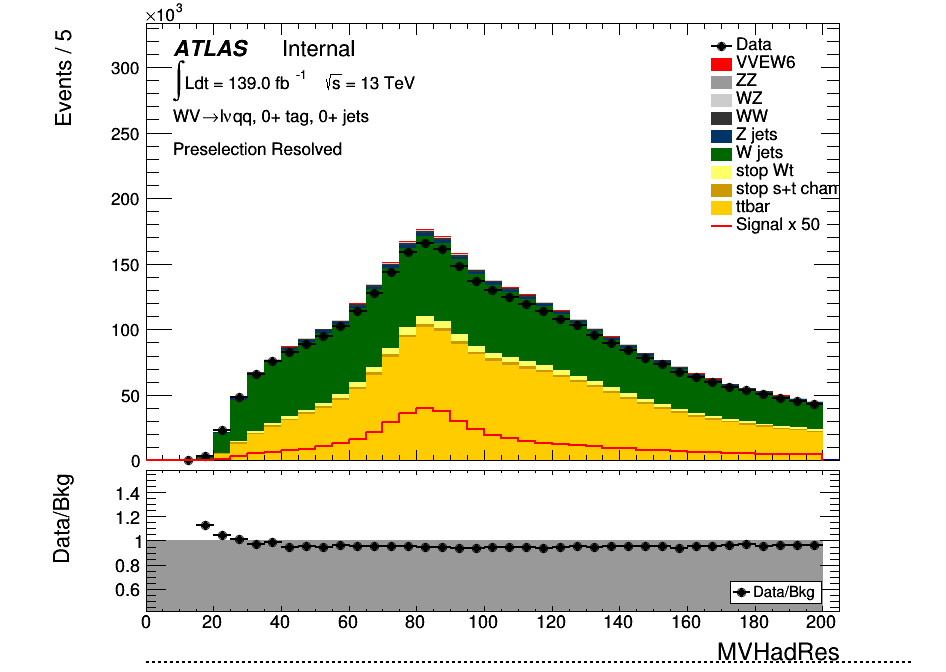
\includegraphics[width=\linewidth]{figures/1lep/CRPlots/C_0ptag0pjet_0ptv_Presel_Resolved_MVHadRes_Lin.png}
        \caption{\emph{\olep}}
    \end{subfigure}
    \begin{subfigure}{0.3\textwidth}
        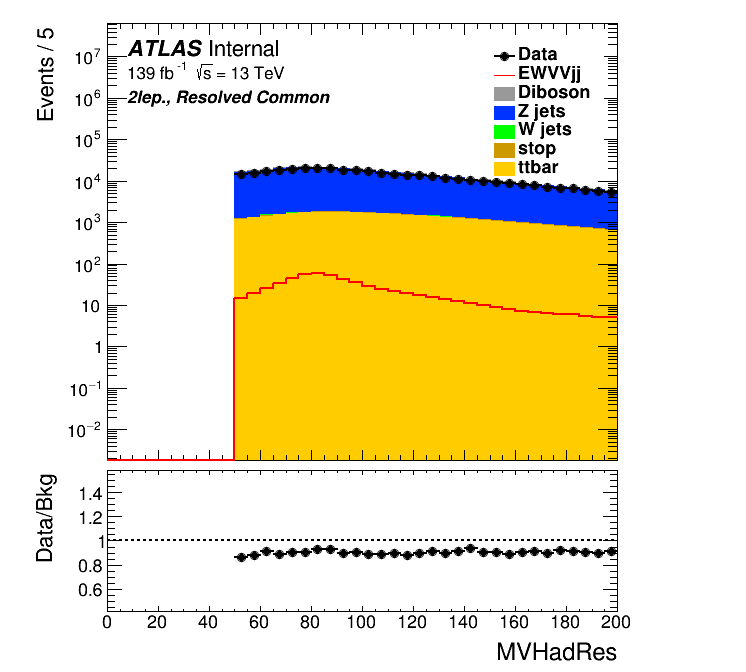
\includegraphics[width=\linewidth]{figures/2lep/dataMC/C_0ptag2pjet_0ptv_ResolvedCommon_MVHadRes_Log.png}
        \caption{\emph{\tlep}}
    \end{subfigure}
    \caption{Mass of reconstructed leading 2 jets in the 1-lepton (left) and 2-lepton channel (right). The plot without mass window cut is shown.}
    \label{fig:1lep2lepMVHadResSR}
\end{figure}


%\begin{figure}[ht]
%    \begin{center}
%        \subfigure[]{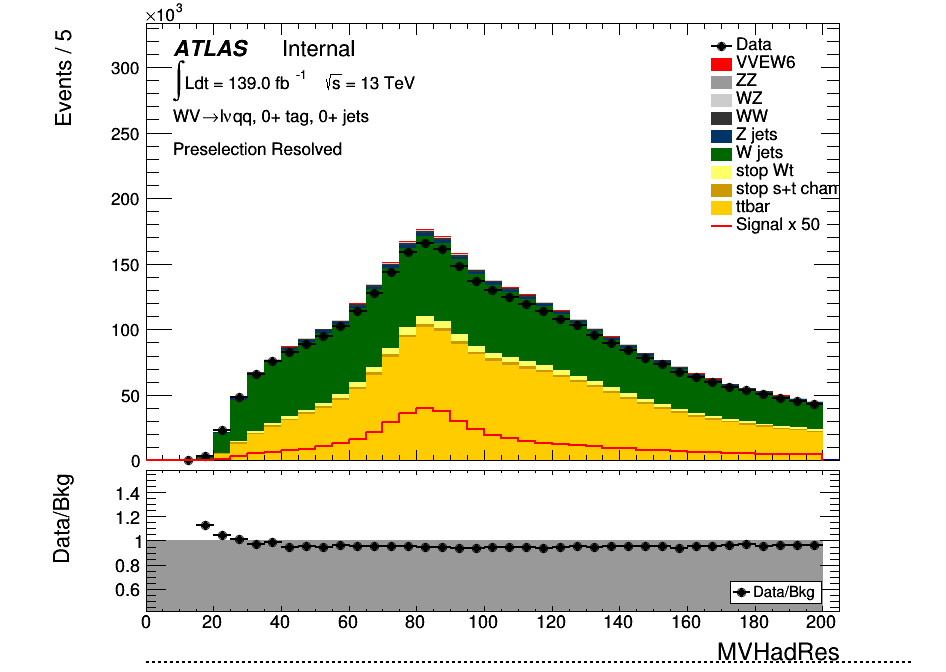
\includegraphics[width=0.3\textwidth]{figures/1lep/CRPlots/C_0ptag0pjet_0ptv_Presel_Resolved_MVHadRes_Lin.png}}
%        \caption{ Mass of reconstructed leading 2 jets in the 1-lepton channel.The plot without mass window cut is shown.}
%    \end{center}
%    \label{fig:1lepMVHadResPresel}
%\end{figure}

\subsection{VV system invariant mass for met associated channels}
\label{subsubsec:mVV_reconstruction}

The mass of the $WV$ system, $m_{WV}$, is calculated using the lepton, neutrino, and the hadronically-decaying boson (represented by either a large-R jet or two small-R jets). To determine the neutrino's momentum in the $z$-direction ($p_z$), we apply the Particle Data Group (PDG) value for the $W$ boson mass to the lepton-neutrino system. This results in a quadratic equation. The solution for $p_z$ is chosen based on the following criteria: if the solutions are complex, we take the real component; if they are real, we select the one with the smaller absolute value.


%%%%%
